\documentclass[varwidth,convert={density=500,size=1080x800,outext=.png}]{standalone}
\usepackage{tikz}
\usetikzlibrary{calc,patterns,decorations.pathmorphing,decorations.markings}
\usepackage{pgfplots}
\usepackage{stanli}

\usepackage[dvipsnames]{xcolor}

\begin{document}
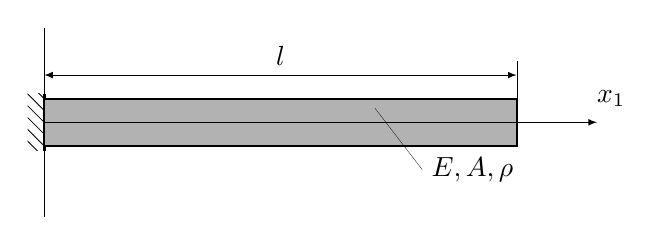
\begin{tikzpicture}[scale=0.6]
	\point{a}{0}{0};
	\support {3}{a}[270];

    % Draw the rectangle
    \filldraw[fill=gray!60, draw=black,thick] (0,-0.5) rectangle (10,0.5);
   
    %axis
    \draw[-latex, ultra thin] (0,0) -- (11.7,0);
    \draw[ultra thin] (0,-2) -- (0,2);
    \node at (12,0.5) {\(x_1\)};
  
    % length
    \draw[ultra thin] (10,0) -- (10, 1.3) ;
    \draw[latex-latex, ultra thin]  (0,1)  to node[sloped,midway,above] {$l$}(10,1) ;
    \draw[ultra thin]  (7,0.3) -- (8,-1) node[right]{$E,A,\rho$};
\end{tikzpicture}    


\end{document}